\subsection{Quantitative Evaluation}\label{sec:quality}
In this part, we quantitatively evaluate our proposals on the \pt{}, \cd{} and \sz{} trajectory datasets from two aspects:
(i) visual quality and (ii) running time.

\begin{figure}[t]
	\centering
	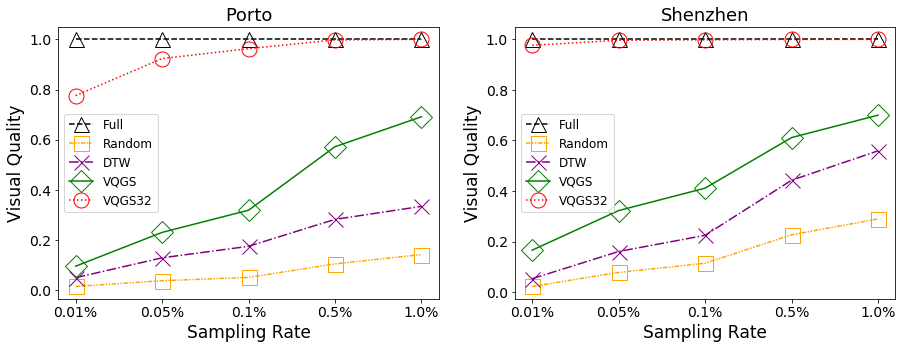
\includegraphics[width=0.5\textwidth]{pictures/quantitative_study_icde/rate_quality.png}
	\vspace{-8mm}
	\caption{Visual quality vs. sampling rates(T1).}
	\label{fig:sample_quality}
	\vspace{-3mm}
\end{figure}

\begin{figure}[t]
	\centering
	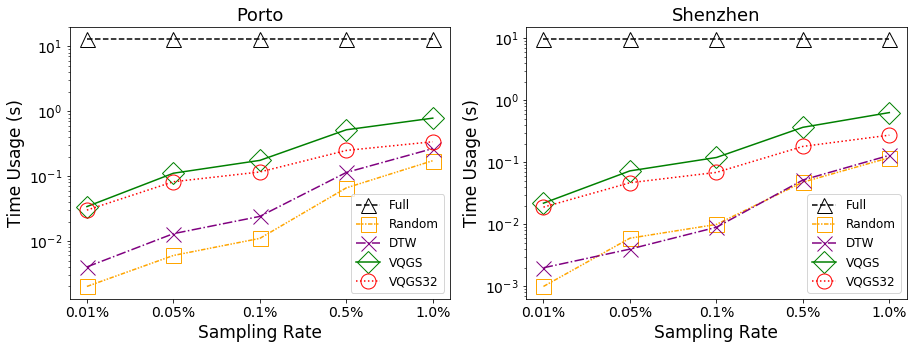
\includegraphics[width=0.5\textwidth]{pictures/quantitative_study_icde/rate_rendertime.png}
	\vspace{-8mm}
	\caption{Rendering time vs. sampling rates(T1).}
	\label{fig:rate_quality}
	\vspace{-3mm}
\end{figure}


\begin{figure}[t]
	\centering
	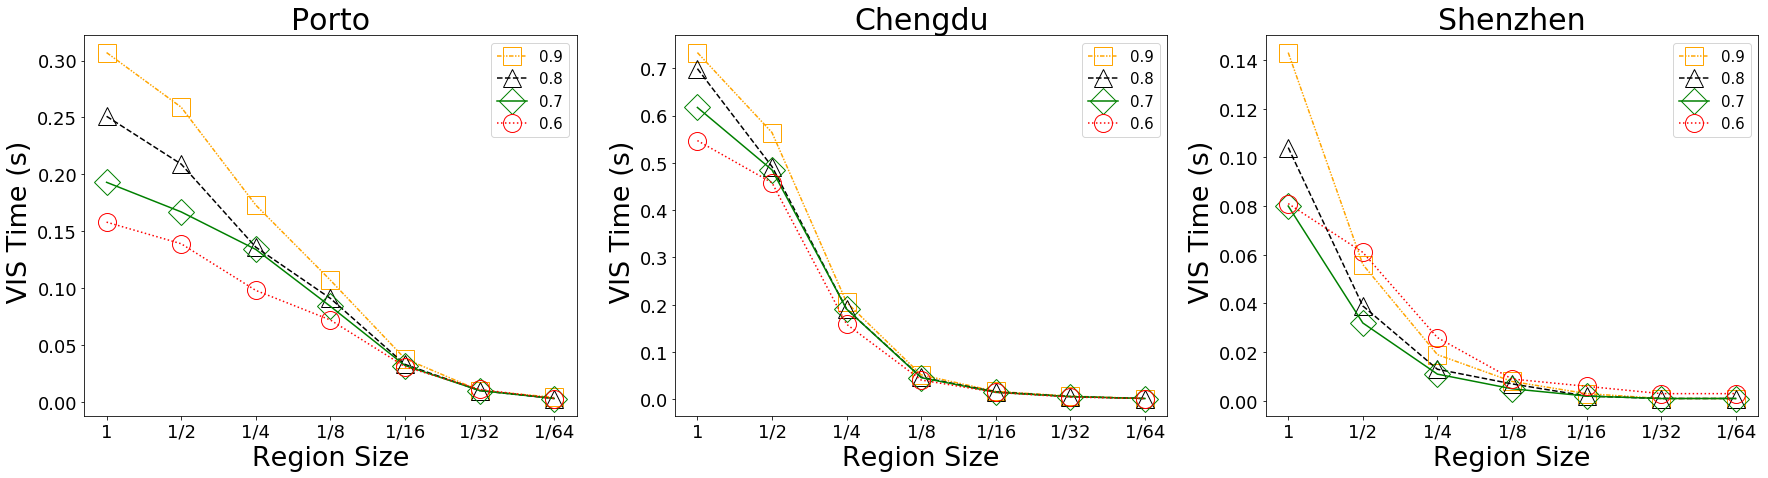
\includegraphics[width=0.5\textwidth]{pictures/quantitative_study_icde/size_rendertime.png}
	\vspace{-8mm}
	\caption{Region size vs. response time(T2).}
	\label{fig:size_rendertime}
	\vspace{-3mm}
\end{figure}

\begin{figure}[t]
	\centering
	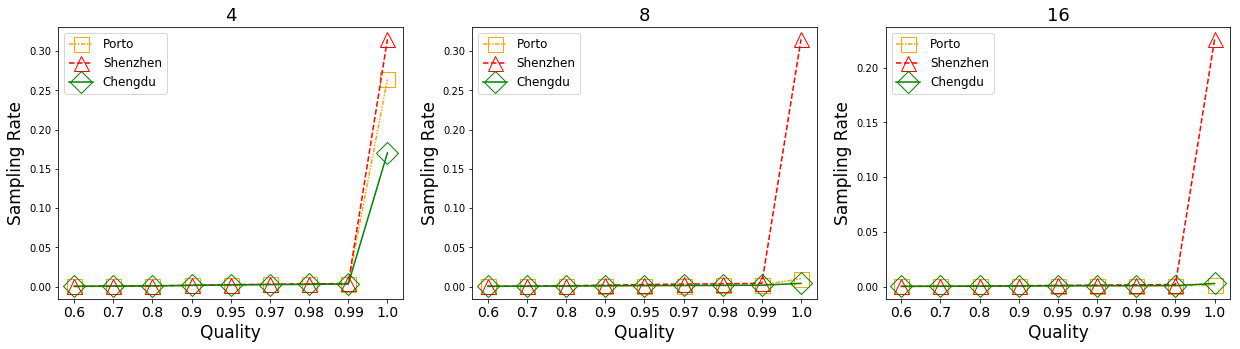
\includegraphics[width=0.5\textwidth]{pictures/quantitative_study_icde/quality_rate.png}
	\vspace{-8mm}
	\caption{Region size vs. response time(T3).}
	\label{fig:quality_rate}
	\vspace{-3mm}
\end{figure}

\begin{figure}[t]
	\centering
	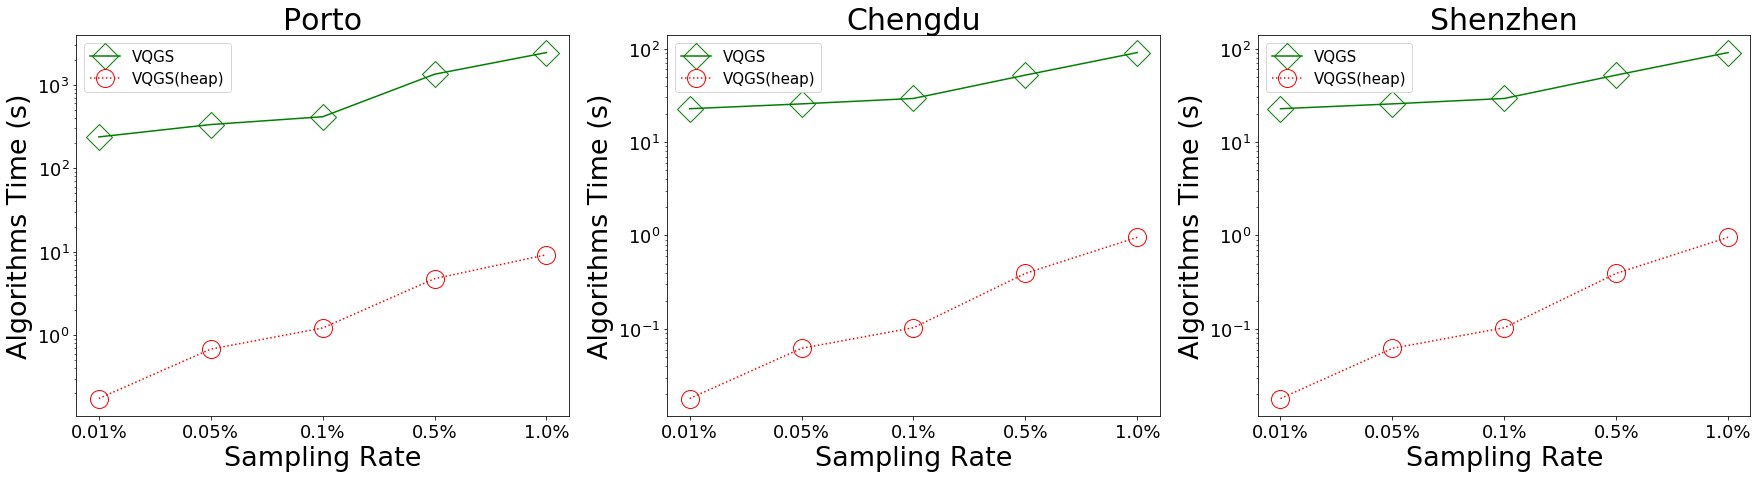
\includegraphics[width=0.5\textwidth]{pictures/quantitative_study_icde/rate_algtime.png}
	\vspace{-8mm}
	\caption{Sampling rate vs. algorithms time(T4).}
	\label{fig:rate_algtime}
	\vspace{-3mm}
\end{figure}
%\begin{figure}[t]
%	\centering
%	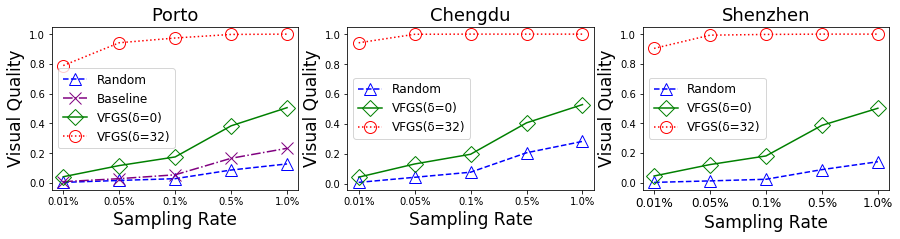
\includegraphics[width=0.5\textwidth]{pictures/quantitative_study_icde/sample_quality.png}
%	\vspace{-8mm}
%	\caption{Visual quality vs. sampling rates.}
%	\label{fig:sample_quality}
%	\vspace{-3mm}
%\end{figure}

%\begin{figure}[t]
%	\centering
%	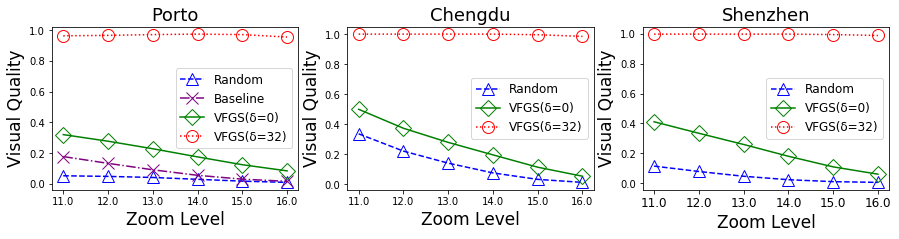
\includegraphics[width=0.5\textwidth]{pictures/quantitative_study_icde/zoom_quality.png}
%	\vspace{-8mm}
%	\caption{Visual quality vs. zoom level.}
%	\label{fig:zoom_quality}
%	\vspace{-3mm}
%\end{figure}

\stitle{Visual quality evaluation}
We evaluate the quality of proposed methods from two aspects: (i) the quality vs different zoom levels; (ii) the quality vs different sampling rates.
Visual quality is defined as the $1-loss$, in which $loss$ is the quality loss function in Equation~\eqref{eqref:loss}. The visualization using the full dataset is used as the ground-truth. 


We report the \textit{visual quality} of different visualization methods in Figure~\ref{fig:sample_quality} with a given sampling $\alpha=0.1\%$. 
The results show that $\rand$ always has the lowest visual quality. $\baseline$ is better than $\rand$ which is also confirmed by case study. Furthermore $\vats$ has better visual quality than $\baseline$ but is significantly outperformed by $\avats$. We also observed that all of the methods across the three dataset have the similar trends: the performance increases when the sampling rate increases.

Figure~\ref{fig:zoom_quality} demonstrates the relationship between visual quality and zoom level. In general, with the increase of the zoom level(zoom into the details), the visual quality drops.
We set the sampling rate $\alpha=1\%$. The results show that $\rand$ always has the lowest  visual quality. $\baseline$ performs better than $\vats$ and $\vats$ is better than $\baseline$. Moreover, $\avats$ has a much higher score than $\vats$. With $\delta=32$ , the minimum visual quality values of $\avats$ are 0.955, 0.985, and 0.989 for \pt{}, \cd{} and \sz{}, respectively. Moreover, the quality of all methods increases when the zoom level drops, which in line with Theorem~\ref{the:level}.



\stitle{Running time evaluation}

%\begin{figure}[t]
%	\centering
%	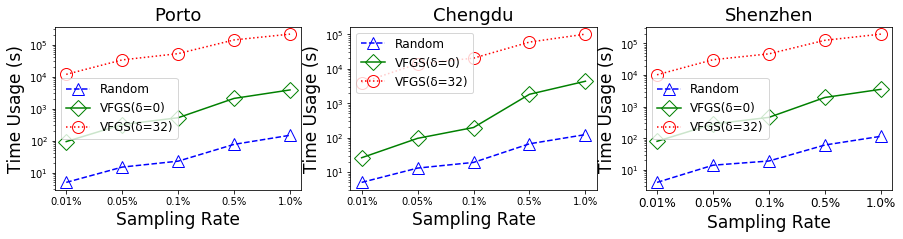
\includegraphics[width=0.5\textwidth]{pictures/quantitative_study_icde/sample_time.png}
%	\vspace{-8mm}
%	\caption{Time usage vs. sampling rates.}
%	\label{fig:sample_time}
%	\vspace{-3mm}
%\end{figure}

%\begin{figure}
%	\centering
%	\small
%	\begin{tabular}{cc}
%		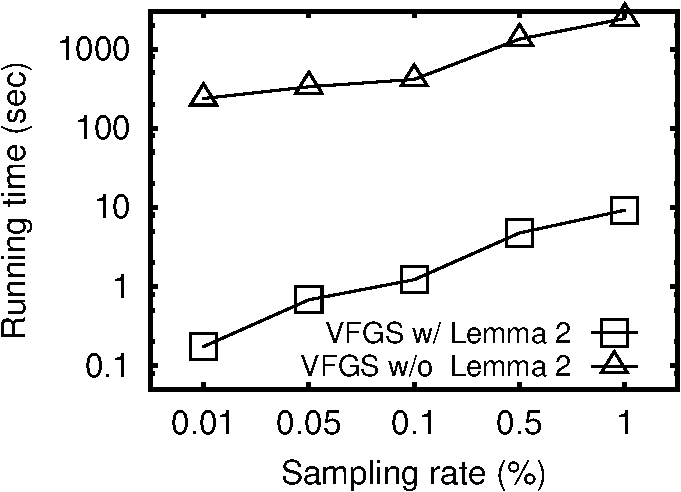
\includegraphics[width=0.44\columnwidth]{pictures/tporto}
%		&
%		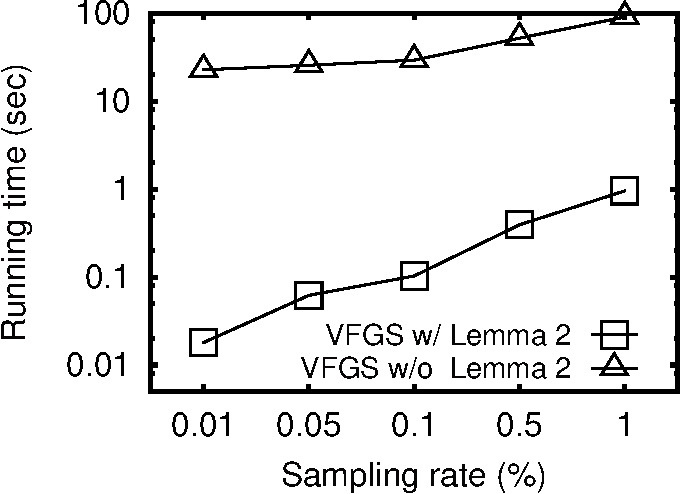
\includegraphics[width=0.44\columnwidth]{pictures/tshenzhen}
%		\\
%		(A) \pt{}
%		&
%		(B) \sz{}	
%	\end{tabular}
%	\vspace{-3mm}
%	\caption{Running time of $\vats$ w/ and w/o Lemma~\ref{lem:submodular}.}
%	\label{fig:cost}
%	\vspace{-6mm}
%\end{figure}
\QM{unfininshed}
We first conduct an experiment to evaluate the rendering cost by datasize. We vary the number of trajectories from 1000 to 1 million, which are randomly selected from \pt{} dataset. The experimental results are summarized in Table~\ref{tab:gpu}. We observe that the rendering cost is linear with the input data trajectories.

We first report the running time of our $\vats$ algorithm in Figure~\ref{fig:cost} by varying the sampling rate from $0.01\%$ to $1\%$. The results show that $\vats$ is quite slow without the submodularity of contribution value, which agrees with Lemma~\ref{lem:submodular} in Section~\ref{sec:opt}.
Then we shown the total time usage with sampling rate as Figure~\ref{fig:sample_time}. {*******}

The optimized $\vats$ (e.g., $\vats$ with Lemma~\ref{lem:submodular}) outperforms $\vats$ by one to three orders of magnitudes on both datasets. The result show that running time of our $\vats$ algorithm is below 1 second in most cases. We have shown that $\vats$ provides good visualization performance with a low sampling rate (e.g., $0.1\%$ or $1\%$) in Section 6.1 and 6.2,  and Table~\ref{tab:gpu} suggests that the rendering latency scales almost linearly with dataset cardinality. By significantly reducing the dataset cardinality with sampling, $\vats$ can effectively reduces the rendering latency to make interactive visualization possible without sacrificing visual quality. For example, rendering the full $\pt{}$ dataset takes about \QM{34 seconds}, with a sampling rate of $1\%$, $\vats$ can bring down the rendering latency to less than 1 second.

\begin{table}
	\centering
	\small
	\caption{Visualization rendering cost}
	\begin{tabular}{|c|c|c|c|c|} \hline
		No. Trajs & GPS points & Mapping (s) & Rendering (s) & Total (s)\\ \hline
		1,000& 31,300 & 0.027 & 0.003 & 0.03 \\ \hline
		10,000& 31,6531 & 0.169 & 0.005 & 0.174\\ \hline
		100,000& 316,7120 & 1.701 & 0.057 & 1.758 \\ \hline
		1,000,000& 31,646,379 & 15.562 & 0.592 & 16.154 \\ \hline
	\end{tabular}	\label{tab:gpu}
\end{table}
